\chapter{Reactive Systems and Asynchronous Programming}\label{chap:rs_reactive_systems_and_asynchronous_programming} % (fold)
\begin{definition}{Reactive System}{react-system}
    A \textbf{reactive system} is a system that computes by reacting to \textit{stimuli} from its environment with asynchronous interactions.
    \begin{note}
        Non-termination can be a feature
    \end{note}
\end{definition}
\textbf{Asynchronous programming} is a main programming style for programming reactive systems.
A style of programming getting more and more importantly today, generally speaking it's about the execution and management of \textbf{asynchronous computations/requests/processes}.
\\
Async panorama:
\begin{itemize}
    \item \textbf{Event-Driven Programming}: event loop based control flow architectures, \textbf{reactor patter};
    \item \textbf{Async Functions \& Continuation Passing Style}: event handlers as continuations, promises library support;
    \item \textbf{Async/await language mechanism}: mimicking synchronous being asynchronous;
    \item \textbf{Coroutine-based Concurrency}: lightweight threads;
\end{itemize}
%
\section{Event-Driven Programming}\label{sec:rs_event_driven_programming} % (fold)
A program is made of routines (\textbf{event handlers}) that are called when \textbf{events} occur.
\begin{note}
    Events can refer to any kind of state's change or input from the environment which is relevant for the program
\end{note}
The control flow of the program depends on events: non-deterministic.
\begin{note}[Aspects]
    \begin{itemize}
        \item How handlers are associated to events;
        \item How events are received and managed;
        \item How handlers are executed;
    \end{itemize}
\end{note}
% section Event-Driven Programming (end)
%
\section{Execution Model: Event Loop}\label{sec:rs_event_loop} % (fold)
In \textbf{Event Loop architectures} a single thread waits for events and executes proper handlers.
An event queue is used to keep track of events generated by either the environment or the event handler themselves.
\begin{codeblock}{}
    loop {
        Event ev = waitForEvent(eventQueue)
        Handler handler = selectHandler(ev)
        execute(handler)
    }
\end{codeblock}
Event handlers are executed \textbf{atomically}: if an event occurs while a handler is in execution, the corresponding event handler is executed only when the handler in execution has completed (\textbf{no concurrency}).
\begin{cimage}
    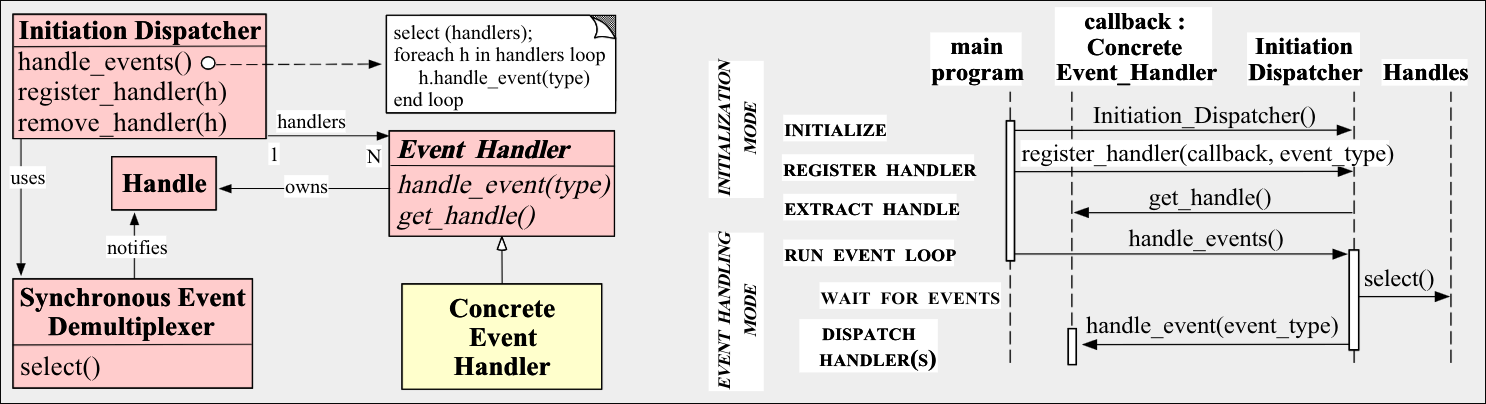
\includegraphics[width=.6\textwidth]{assets/20261116_135321.png}
    \caption{Reactor Pattern}\label{fig:20261116_135321}
\end{cimage}
%
\paragraph{Multiple Event Loops}\label{par:rs_multiple_event_loops} % (fold)
Conceptually, an event-loop can be used as the control architecture of a single active component:
\begin{itemize}
    \item event-driven behavior;
    \item private event queue;
    \item asynchronous non-blocking \hyperref[def:task]{Tasks};
\end{itemize}
A system can be composed by \textbf{multiple active components} each one with its own event-loop:
\begin{itemize}
    \item non-sharing memory;
    \item interacting by generating \textbf{events};
\end{itemize}
% paragraph Multiple Event Loops (end)
%
\subsection{Never Blocking Rule and Concurrency}\label{sub:rs_never_blocking_rule_and_concurrency} % (fold)
The execution model leads to an important rule in designing/programming event handlers.
\begin{quote}
    Event handlers \textbf{should never block} (should not contain blocking calls) and should always terminate (must not contain infinite loops)
\end{quote}
This is to guarantee responsiveness of the system: a blocking call or infinite loop would block the \hyperref[sec:rs_event_loop]{Event Loop} serving the events and events in queue would not be processed.
Also, a blocking call must be replaced by an asynchronous request or computation, which will eventually generate some event in the future (result or error):
\begin{itemize}
    \item asynchronous requests/tasks are served by other threads, independent of the \hyperref[sec:rs_event_loop]{Event Loop};
    \item these threads interact with the \hyperref[sec:rs_event_loop]{Event Loop} by inserting events in the event queue;
\end{itemize}
% subsection Never Blocking Rule and Concurrency (end)
% section Execution Model: Event Loop (end)
%
\section{Callback Model}\label{sec:rs_callback_model} % (fold)
Given the \hyperref[sub:rs_never_blocking_rule_and_concurrency]{Non-Blocking Rule}, a main issue is:
\begin{quote}[How to execute long-running handlers, without blocking and tampering reactivity?]
    By executing asynchronous \hyperref[def:task]{Tasks}/functions: the handler triggers the execution of an async \hyperref[def:task]{Task}/function and goes on, without waiting for the result (or error)
\end{quote}
\begin{warning}[Problem]
    How to process results or errors that are asynchronously generated by the async \hyperref[def:task]{Task}/function execution?
    \begin{tip}[Callback Model]
    \end{tip}
\end{warning}
\begin{definition}{Callback Model}{callback-model}
    A function, called \textbf{callback}, is specified as an argument of the async \hyperref[def:task]{Task}/function call.
    The callback is called by the \hyperref[sec:rs_event_loop]{Event Loop} when processing the event related to the result or error generated by the async \hyperref[def:task]{Task}/function execution.
    \begin{note}
        It's a kind of ``implicit'' handler registered dynamically to the event corresponding to the result/error
    \end{note}
\end{definition}
\begin{note}
    In this way the callback defines a ``continuation'' of the computation (\textbf{\ac{cps}})
\end{note}
%
\subsection{Continuation Passing Style}\label{sub:rs_continuation_passing_style} % (fold)
In \red{functional programming}, \acf{cps} is a style of programming in which control is passed explicitly in the form of a \textbf{continuation}.
\begin{definition}{Continuation Passing Style}{cps}
    A function written in \textbf{continuation-passing style} takes an extra argument: a \textbf{function} of one argument (\textit{the continuation}).
    When the \ac{cps} function has computed its result value, it ``return'' it by calling the continuation function with this value as the argument, so the stack is not used.
    \begin{note}[Actually]
        When invoking a \ac{cps} function, the calling function is required to supply a procedure to be invoked with the subroutine's ``return'' value
    \end{note}
    \begin{codeblock}[java]{}
    void sum(x, y, cont) {
        cont(x + y);
    }

    sum(1, 3, (res) -> print(res));
    \end{codeblock}
\end{definition}
\paragraph{Callbacks as Continuations}\label{par:rs_callbacks_as_continuations} % (fold)
Callbacks are like \textit{continuations} that are called when the result of the asynchronous computation is ready.
\begin{example}{}{}
    \begin{codeblock}[js]{Synch Version}
    function loadUserPic(userId) {
        let user = findUserById(userId);
        return loadPic(user.picId);
    }
    \end{codeblock}
    \begin{codeblock}[js]{Async Version}
    function loadUserPic(userId, ret) {
        findUserById(userId, (user) => {
            loadPic(user.picId, ret);
        });
    }

    loadUserPic('john', (pic) => {
        ui.show(pic);
    });
    \end{codeblock}
\end{example}
\begin{note}[Using Closures as Callbacks]
    Callbacks are often implemented as \textit{closures}: technique for implementing lexically scoped name binding in a language with first-class functions.
    Operationally, a \textbf{closure} is a record storing a function together with an environment:  the environment is a mapping associating each free variable of the function with the value or reference to which the name was bound when the closure was created.
\end{note}
% paragraph Callbacks as Continuations (end)
% subsection Continuation Passing Style (end)
%
\subsection{Callback Execution Model}\label{sub:rs_callback_execution_model} % (fold)
\begin{quote}
    A main question is: \textit{who invokes the continuation/callback?}
\end{quote}
Two main possibilities:
\begin{itemize}
    \item a thread of control \textbf{different from the thread} that triggered the request;
        \begin{warning}[Race conditions]
        \end{warning}
    \item in \hyperref[sec:rs_event_driven_programming]{Event-Driven} architectures based on the  \hyperref[sec:rs_event_loop]{Event Loop Model}, the \textbf{continuation is executed by the  \hyperref[sec:rs_event_loop]{Event Loop}};
\end{itemize}
\begin{note}[Callbacks as Continuations]
    In this case:
    \begin{itemize}
        \item events are implicit and refer to the completion with success or error of an asynchronous request/computations;
        \item event handlers are represented by continuation functions specified when invoking the asynchronous request/computation;
        \item closures are typically used to define the context to be used when processing the event;
    \end{itemize}
\end{note}
\begin{example}{JavaScript Client}{}
    Event-loop ruling script execution.
    \begin{codeblock}[js]{Non Blocking I/O}
    let ajaxRequest = new XMLHttpRequest;
    ajaxRequest.open('GET',url);
    ajaxRequest.send(null);
    ajaxRequest.onreadystatechange =
    function() {
        // what to do next
    }
    \end{codeblock}
    \begin{codeblock}[js]{Wrong Way of doing it}
    // this is wrong
    let ajaxRequest = new XMLHttpRequest;
    ajaxRequest.open('GET',url);
    ajaxRequest.send(null);
    while (ajaxRequest.readyState === XMLHttpRequest.UNSENT) {}
    // !DEADLOCK!
    \end{codeblock}
    The method \texttt{setTimeout(callback, timeout)} is another asynchronous function, registering a callback to be executed when the timeout expires.
    \begin{codeblock}[js]{}
    var sys = require("sys"),
    http = require("http"),
    url = require("url"),
    path = require("path"),
    fs = require("fs");
    http.createServer((request, response) => {
        let uri = url.parse(request.url).pathname;
        let filename = path.join(process.cwd(), uri);
        path.exists(filename, (exists) => {
            if(exists) {
                fs.readFile(filename, (err, data) => {
                    response.writeHead(200);
                    response.end(data);
                });
            } else {
                response.writeHead(404);
                response.end();
            }
        });
    }).listen(8080);
    sys.log("Server running at http://localhost:8080/");
    \end{codeblock}
\end{example}
% subsection Callback Execution Model (end)
% section Callback Model (end)
%
\section{Continuation-Based Asynchronous Programming}\label{sec:rs_continuation_based_asynchronous_programming} % (fold)
Using a \textbf{single thread} to coordinate and manage multiple asynchronous \hyperref[def:task]{Task}:
\begin{itemize}
    \item eventually executed by external/OS-backed threads;
    \item low memory footprint compared to multithreaded solutions;
    \item based on an implicit \hyperref[sec:rs_event_loop]{Event Loop};
\end{itemize}
\begin{note}[No low-level races and low-level deadlocks]
\end{note}
\begin{description}
    \item[Problems] Besides the benefits, there are some main well-known problems affecting \hyperref[def:cps]{CPS} and \hyperref[sec:rs_event_driven_programming]{Event-Driven Programming}, often referred altogether as \textit{callback hell}:
        \begin{itemize}
            \item \textbf{asynchronous spaghetti}, overall computation fragmented into asynchronous handlers, this tampers the modularity and structure of programs making them difficult to understand and maintain;
            \item \textbf{pyramid of doom/callback hell}, composition based on \hyperref[def:cps]{CPS} leads to nested callbacks/continuations, this increases complexity and leads to poor source code readability, bad reusability, bad extendibility;
                \begin{codeblock}[js]{Callback Nesting = Pyramid of Doom or Callback Hell}
    step1(function(result1)) {
        step2(function(result2)) {
            step3(function(result3)){
                // and so on...
            }
        }
    }
                \end{codeblock}
        \end{itemize}
\end{description}
%
\subsection{Promises}\label{sub:rs_promises} % (fold)
The \red{callback hell} can be partially solved by adopting the \textbf{promise} mechanism.
\begin{definition}{Promises}{promises}
    \textbf{Promises} represent the \textbf{eventual completion} and \textbf{result} of a single asynchronous operation.
    They encapsulate asynchronous actions, acting much like a value returned from the result of a computation only that the value may not be available at the time.
    \begin{warning}
        A promise can be \textbf{rejected} or \textbf{resolved} once and only once: immutable once-resolved promises
    \end{warning}
    \begin{note}[Key Property]
        They allow flattening callback nesting
    \end{note}
\end{definition}
\begin{example}{}{}
    \begin{codeblock}[js]{}
    let promisedPic = loadUserPic('john');

    promisedPic.then((pic) => {
        ui.show(pic);
    });
    \end{codeblock}
\end{example}
An operation that may take some time to return a \texttt{Promise} object at once and then complete its \hyperref[def:task]{Task} in background (async):
\begin{codeblock}[js]{}
    let myPromise = asyncFunc(args);
\end{codeblock}
Promise is regarded as being a Promise to deliver a future value, we can configure the \texttt{Promise} to specify what should happen when the \texttt{asyncFunc} is complete.
\begin{codeblock}[js]{}
    myPromise.then(onComplete, onError);
\end{codeblock}
\begin{itemize}
    \item \texttt{onComplete} is a callback called if/when the \texttt{asyncFunc} is complete;
    \item \texttt{onError} (optional) is a callback called if/when the \texttt{asyncFunc} produced an error;
\end{itemize}
%
\subsubsection{Promise Object}\label{sub:rs_promise_object} % (fold)
A Promise object can be in one of three states:
\begin{itemize}
    \item \textbf{pending}: when the \texttt{Promise} is first created;
    \item \textbf{resolved} (or fulfilled): if the async function/\hyperref[def:task]{Task} ends correctly;
    \item \textbf{rejected}: if the async function/\hyperref[def:task]{Task} ends with an error;
\end{itemize}
\begin{note}
    It is also called \textbf{settled} if it isn't pending: it's either resolved or rejected.
    Once a Promise is \textbf{settled}, its state and value doesn't change.
\end{note}
\begin{example}{Promise Definition and Usage}{}
    \begin{codeblock}[js]{}
    function delayWithRandom(t,p){
        let promise = new Promise((resolve,reject) => {
            setTimeout(() => {
                let r = Math.random();
                if (r > p) {
                    resolve(r);
                } else {
                    reject(r);
                }
            },t);
        });
        return promise;
    }

    let promise = delayWithRandom(1000,0.5);
    promise.then((r) => {
        console.log("success: ",r);
    },(r) => {
        console.log("fail: ",r);
    });
    \end{codeblock}
\end{example}
% subsubsection Promise Object (end)
%
\subsubsection{Promise Chaining}\label{sub:rs_promise_chaining} % (fold)
Key feature for flattering the \textbf{pyramid of doom}, \textit{then} method returns itself a promise, so that promises can be chained.
\begin{codeblock}[js]{}
    let promise = new Promise((resolve, reject) => {
        resolve(1);
    });
    promise.then((val) => {
        console.log(val); // 1
        return val + 2;
    }).then((val) => {
        console.log(val); // 3
    });
\end{codeblock}
The value of each \hyperref[def:promises]{Promise} in a chain is whatever the previous \texttt{onComplete/onError} returns.
\begin{codeblock}[js]{}
    let myProm1 = delayWithRandom(1000,0.5);
    let myProm2 = myProm1.then((v) => {
        console.log(v);
        return "done";
    });
    myProm2.then((v) => {
        console.log(v);
    });
\end{codeblock}
%
\paragraph{Chaining Async Functions}\label{par:rs_chaining_async_functions} % (fold)
To chain async functions, not only the first generating \hyperref[def:promises]{Promise}, we can return \hyperref[def:promises]{Promises} in the chain.
\begin{codeblock}[js]{}
    function delayWithRand(t){
        let promise = new Promise((resolve,reject) => {
            setTimeout(() => {
                var r = Math.random();
                resolve(r);
            },t);
        });
        return promise;
    }

    let promise = delayWithRand(1000);
    promise.then((r) => {
        console.log("success: ",r);
        return delayWithRand(1500);
    }).then((r) => {
        console.log("success: ",r);
        return delayWithRand(500);
    }).then((v) => {
        console.log(v);
    });
\end{codeblock}
% paragraph Chaining Async Functions (end)
% subsubsection Promise Chaining (end)
%
\subsubsection{Parallel Execution}\label{sub:rs_pr_parallel_execution} % (fold)
Both callbacks are called when \texttt{asyncFunc1} ends, with the same value hold by the \hyperref[def:promises]{Promise}.
\begin{codeblock}[js]{}
    let myPromise = asyncFunc1();
    myPromise.then((v) => {
        console.log(v);
        return asyncFunc2();
    });
    myPromise.then((v) => {
        console.log(v);
        return asyncFunc3();
    });
\end{codeblock}
% subsubsection Parallel Execution (end)
%
\subsubsection{Combining Promises -- All}\label{sub:rs_combining_promises_all} % (fold)
Composing a set of independent asynchronous calls, to be executed in parallel with a join point.
\begin{codeblock}[js]{}
    let totalProm = Promise.all(promiseList);
    totalProm.then(function(values){})
\end{codeblock}
The callback is called when all \hyperref[def:promises]{Promises} are resolved or at least rejected.
\begin{example}{}{}
    \begin{codeblock}[js]{}
    let myProm1 = delayWithRand(1000);
    let myProm2 = delayWithRand(2000);
    let myTotalProm = Promise.all([myProm1, myProm2]);
    myTotalProm.then((values) => {
        console.log(values[0]);
        console.log(values[1]);
    });
    \end{codeblock}
\end{example}
% subsubsection Combining Promises -- All (end)
%
\subsubsection{Combining Promises -- Race}\label{sub:rs_combining_promises_race} % (fold)
Composing a set of independent asynchronous calls, but completing as soon as one completes.
\begin{codeblock}[js]{}
    let totalProm = Promise.race(promiseList);
    totalProm.then(function(value){},
    function(value){});
\end{codeblock}
The callback is called when a \hyperref[def:promises]{Promise} is resolved or rejected.
\begin{example}{}{}
    \begin{codeblock}[js]{}
    let myProm1 = delayWithRand(1000);
    let myProm2 = delayWithRand(2000);
    let myTotalProm = Promise.race([myProm1, myProm2]);
    myTotalProm.then((value) => {
        console.log(value);
    });
    \end{codeblock}
\end{example}
% subsubsection Combining Promises -- Race (end)
%
\subsubsection{Promise Error Handling}\label{sub:rs_promise_error_handling} % (fold)
\begin{note}[Rules]
    \begin{itemize}
        \item any handler that returns a value and does not throw an error passes on success to the next \hyperref[def:promises]{Promise}, including \texttt{onFailure} handlers;
        \item any handler that throws an exception passes a \textbf{reject} on the next \hyperref[def:promises]{Promise};
        \item an unhandled state is passed to the next \hyperref[def:promises]{Promise} in the chain:
            \begin{itemize}
                \item if there is no rejection handler and the \hyperref[def:promises]{Promise} is \textbf{rejected} then the state is passed to the next handler in the chain;
                \item once the state has found a handler then processing resumes its normal handler in the chain;
                \item similar to the synchronous case;
            \end{itemize}
    \end{itemize}
\end{note}
% subsubsection Promise Error Handling (end)
%
\subsubsection{Immediately Resolve}\label{sub:rs_immediately_resolve} % (fold)
\texttt{Promise.resolve} API to build \hyperref[def:promises]{Promises} that can be immediately resolved, then can be used to chain a callback to be executed in next cycle of the \hyperref[sec:rs_event_loop]{Event Loop}.
\begin{codeblock}[js]{}
    console.log("this cycle");
    Promise
    .resolve("done")
    .then(() => {
        console.log("next cycle");
    });
\end{codeblock}
% subsubsection Immediately Resolve (end)
%
\subsubsection{Tasks and Microtasks}\label{sub:rs_tasks_and_microtasks} % (fold)
In JavaScript and Web world, the event queue, also called \textbf{dispatch queue}, hosts both \hyperref[def:task]{Tasks} and \textit{microtasks}.
The event loop works as usual:
\begin{itemize}
    \item takes \hyperref[def:task]{Tasks} one at a time and allows the \hyperref[def:task]{Task} to run to completion before the next \hyperref[def:task]{Task} is serviced;
    \item \hyperref[def:task]{Tasks} can also be preferentially dequeued (priorities);
\end{itemize}
Micro \hyperref[def:task]{Tasks} has been introduced as a lightweight version of the \hyperref[def:task]{Task}.
They are guaranteed to be executed before the next \hyperref[def:task]{Task} starts, the microtasks queue is processed after each \hyperref[def:task]{Task} starts.
\begin{codeblock}[js]{}
    Promise.resolve().then(() => {});
\end{codeblock}
\begin{cimage}
    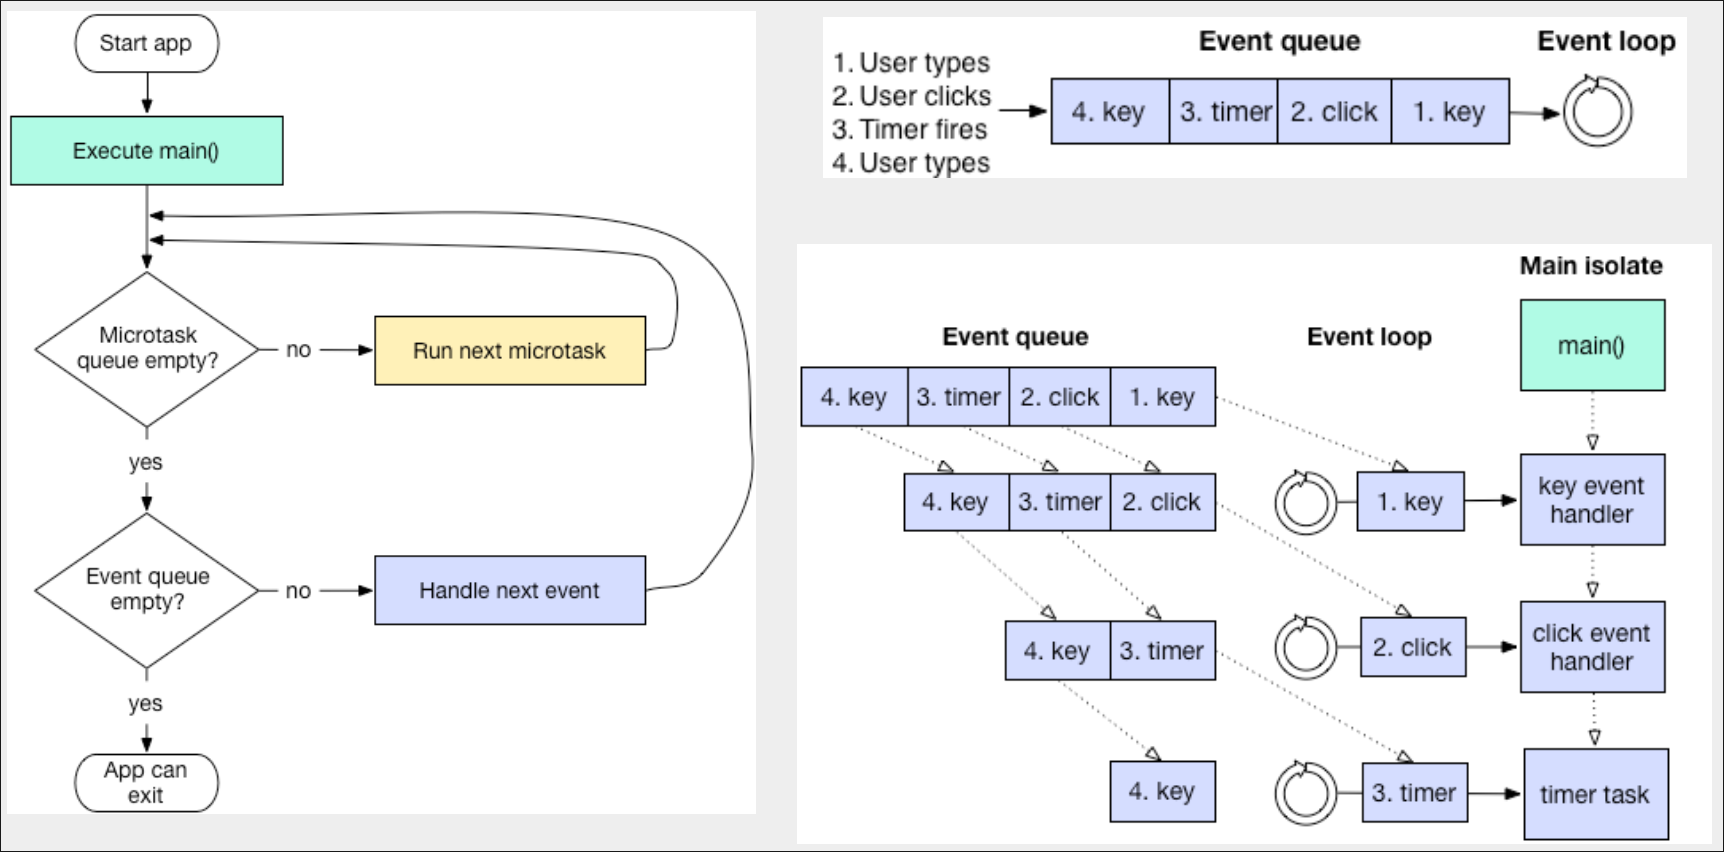
\includegraphics[width=.6\textwidth]{assets/20261120_143058.png}
\end{cimage}
\begin{note}
    While the event loop is executing \hyperref[def:task]{Tasks} from the microtask queue, the event queue is stuck: the app can't draw graphics, handle mouse clicks, rect to I/O, and so on
\end{note}
% subsubsection Tasks and Microtasks (end)
%
\subsubsection{The Problem with Promises}\label{sub:rs_the_problem_with_promises} % (fold)
\begin{multicols}{2}
    \begin{itemize}
        \item we cannot pass parameters to functions used in a \texttt{then} block;
        \item they cannot be used with loops or iterations;
        \item they cannot be cancelled, and we have no control over the async \hyperref[def:task]{Task};
        \item they are \textbf{eager}: when they are constructed they immediately begin to work;
    \end{itemize}
\end{multicols}
% subsubsection The Problem with Promises (end)
% subsection Promises (end)
%
\subsection{From Promises to Async/Await}\label{sub:rs_from_promises_to_async_await} % (fold)
The language extension \textbf{async} \& \textbf{await} is the most recent and promising solution in async programming.
\begin{note}[Idea]
    The goal is to provide a \textbf{synch} programming style while keeping an \textbf{asynchronous core}.
\end{note}
\begin{codeblock}[js]{}
    let p = asyncFunc();
    let res = await p;
    // <use res>
\end{codeblock}
\begin{quote}
    Conceptually wait for \texttt{asyncFunc} result (yielding the control) and then continue with the program (getting back the control) when the \hyperref[def:promises]{Promise} is solved
\end{quote}
%
\subsubsection{Await Operator}\label{sub:rs_await_operator} % (fold)
\begin{codeblock}[js]{}
    await promise;
\end{codeblock}
Can be applied to any \hyperref[def:promises]{Promise}, and it \textbf{suspends the function execution} until the \hyperref[def:promises]{Promise} is fulfilled.
\begin{critical}[It does NOT block the control flow]
    The control flow is \textbf{yield}, saving the current computation state
\end{critical}
It can be used only in the body of functions labelled as \textbf{async}:
\begin{codeblock}[js]{}
    async function f() {}

    async function f1() {
        await f();
    }
\end{codeblock}
% subsubsection Await Operator (end)
%
\subsubsection{Async Functions}\label{sub:rs_async_functions} % (fold)
A \texttt{async} function is a suspendible function returning a \hyperref[def:promises]{Promise}.
\begin{codeblock}[js]{}
    var myFunc = async () => {
        return 1 + 2;
    }
\end{codeblock}
The function is converted into an \texttt{AsyncFunction} object function: the function is just defined not executed.
By calling the function, the code is executed as a normal function, in the same cycle, returning a \hyperref[def:promises]{Promise}.
\begin{cimage}
    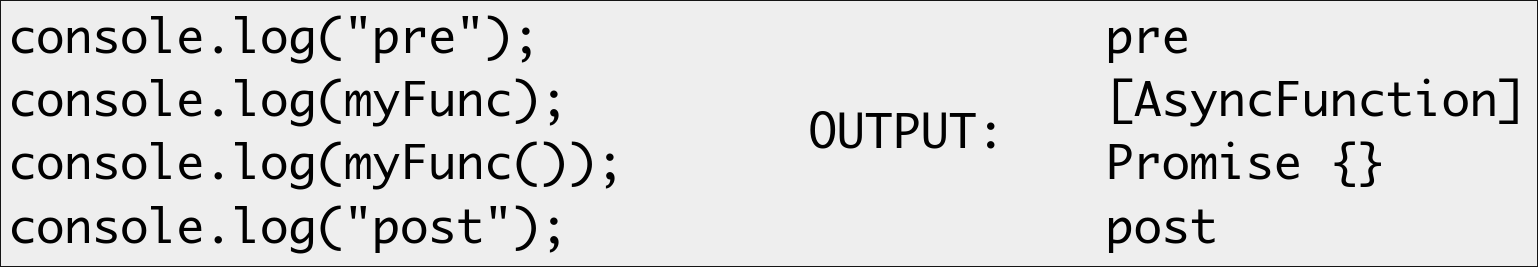
\includegraphics[width=.6\textwidth]{assets/20261120_152510.png}
\end{cimage}
An \texttt{AsyncFunction} object contains the low-level machinery, based on co-routines, to allow for expressing the body of the asynchronous function using a synchronous style.
\begin{warning}
    Async functions can be called either with \texttt{await} or not, producing a different behavior.
    \begin{codeblock}[js]{}
    async function pause(t){
        console.log("before");
        let promise = new Promise((resolve, reject) => {
            setTimeout(() => resolve() ,t);
        });
        await promise;
        console.log("after");
    }
    \end{codeblock}
    \begin{codeblock}[js]{Without}
    console.log("before call");
    pause(1000);
    console.log("after call");
    \end{codeblock}
    \begin{codeblock}[js]{With}
    async function main(){
        console.log("before call");
        await pause(1000);
        console.log("after call");
    }
    main();
    \end{codeblock}
\end{warning}
% subsubsection Async Functions (end)
%
\subsubsection{Await Details}\label{sub:rs_await_details} % (fold)
The \texttt{await promise} converts a \hyperref[def:promises]{Promise} into a result or an exception just as if it was a result from a \textbf{synchronous function}.
If the \hyperref[def:promises]{Promise} is resolved, the \texttt{await} operator extracts the resolved value and returns it; if the \hyperref[def:promises]{Promise} is rejected then the \texttt{await} throws an exception with the rejected value.
% subsubsection Await Details (end)
% subsection From Promises to Async/Await (end)
%
\subsection{Co-Routines}\label{sub:rs_co_routines} % (fold)
\hyperref[sub:rs_await_operator]{Await} behave like a return that can be resumed: when a function executes an \texttt{await}, the thread returns to the calling program which receives the \hyperref[def:promises]{Promise} object created by the \hyperref[sub:rs_async_functions]{Async Function} in a \textbf{pending} state.
The state of the computation is saved, to be restored when the \textbf{control} is back.
The \hyperref[sub:rs_async_functions]{Async Function} is resumed asynchronously, as soon as the \hyperref[sec:rs_event_loop]{Event Loop} thread fetches the corresponding event in the \textbf{event queue}.
\emptyln{}
To release and resume the control in the implementation of \textit{await/async}, the \textbf{co-routine} mechanism is exploited:
\begin{itemize}
    \item old mechanisms adopted for cooperative scheduling;
    \item brought back in asynchronous programming based on a single control flow;
\end{itemize}
\begin{note}[Benefits]
    Asynchronous programming is greatly simplified: no need to explicitly use \hyperref[def:promises]{Promises}/then/chains for implementing the sequence execution pattern.
    \\
    The eagerness \& then pattern problem are solved, and they can be used with loop or iterations.
    \begin{codeblock}[js]{}
    async function waitFor(t){
        console.log("waitFor - pre");
        await delay(t);
        console.log("waitFor - post");
    }
    async function main(){
        console.log("Before");
        for (let i = 0; i < 3; i++){
            await waitFor(1000);
            console.log("Step " + i);
        }
        console.log("After");
    };
    \end{codeblock}
\end{note}
\begin{critical}[Issues]
    Some issues affecting async/wait:
    \begin{itemize}
        \item await can be used only inside an \hyperref[sub:rs_async_functions]{Async Function} body, but it cannot be used at the top level: it needs to introduce at least one main \hyperref[sub:rs_async_functions]{Async Function};
        \item an \hyperref[sub:rs_async_functions]{Async Function} cannot resume while the thread is busy running other handlers: the \hyperref[sec:rs_event_loop]{Event Loop} semantics is preserved;
        \item \textbf{blocks \texttt{\{\dots\}}} are no more guaranteed to be atomic: the execution of the code of a single block can span over multiple iterations of the  \hyperref[sec:rs_event_loop]{Event Loop} (\hyperref[def:race-cond]{Race Conditions});
    \end{itemize}
    \begin{example}{Composing Issue}{}
        Needs to mix await/async with \hyperref[def:promises]{Promises}
        \begin{codeblock}[js]{}
        async function f(){
            await delay(1000);
            return 1 + 2;
        }
        async function g(){
            await delay(5000);
            return 2 + 3;
        }
        async function compose(){
            console.log("before");
            let r = await Promise.all([f(), g()]);
            console.log("done: " + r);
        }
        compose();
        \end{codeblock}
    \end{example}
    \begin{note}[Design Clash Issue]
        Design clash between synchronous and asynchronous: strong discipline needed in mixing sync/async style to avoid programs whose behavior is difficult to understand
        \begin{tip}
            Need of higher level of abstractions/concepts that naturally integrate a sync and an async perspective
        \end{tip}
    \end{note}
\end{critical}
Generalization of the subroutine concept by allowing \textbf{execution} to be \textbf{suspended} and \textbf{resumed}:
\begin{itemize}
    \item for non-preemptive, cooperative multitasking;
    \item basic building block for implementing cooperative \hyperref[def:task]{Tasks}, exceptions, \hyperref[sec:rs_event_loop]{Event Loops}, iterators, infinite lists and pipes;
    \item not related to events and \hyperref[sec:rs_event_driven_programming]{Event-Driven Programming};
\end{itemize}
%
\subsubsection{Coroutines as Generalized Routine}\label{sub:rs_coroutines_as_generalized_routine} % (fold)
When calling a \hyperref[sub:rs_co_routines]{Coroutine} can exit by calling other \hyperref[sub:rs_co_routines]{Coroutines}, which may later return to the point where they were invoked in the original \hyperref[sub:rs_co_routines]{Coroutine}:\begin{itemize}
    \item from the \hyperref[sub:rs_co_routines]{Coroutine}'s point of view, it is not exiting but \textit{calling another \hyperref[sub:rs_co_routines]{Coroutine}};
    \item calling another \hyperref[sub:rs_co_routines]{Coroutine} can be done by ``yielding'' to it;
\end{itemize}
\begin{codeblock}[txt]{A Cooperative one-flow based Producer Consumer System}
    var q := new queue

    coroutine produce
        loop
            while q is not full
                create some new items
                add the items to q
            yield to consume

    coroutine consume
        loop
            while q is not empty
                remove some items from q
                use the items
            yield to produce
\end{codeblock}
% subsubsection Coroutines as Generalized Routine (end)
%
\subsubsection{Coroutine Characteristics}\label{sub:rs_coroutine_characteristics} % (fold)
A \hyperref[sub:rs_co_routines]{Coroutine} instance holds state, and varies between invocations: there can be multiple instances of a given \hyperref[sub:rs_co_routines]{Coroutine} at once.
Traditional \textit{subroutines} are special cases of \hyperref[sub:rs_co_routines]{Coroutines} where any subroutine can be translated to a \hyperref[sub:rs_co_routines]{Coroutine} which does not call \textit{yield}.
\emptyln{}
They can be easily implemented just as a library on top of a language based on just subroutines and subroutine-like mechanism.
% subsubsection Coroutine Characteristics (end)
% subsection Co-Routines (end)
% section Continuation-Based Asynchronous Programming (end)
%
\section{Concurrency Model Based on Coroutines}\label{sec:rs_concurrency_model_based_on_coroutines} % (fold)
\hyperref[sub:rs_co_routines]{Coroutines} can be used as low-level mechanism to implement \red{lightweight threads}.
One thread can have many \hyperref[sub:rs_co_routines]{Coroutines} inside it, but only one \hyperref[sub:rs_co_routines]{Coroutine} is in execution at a given time
\begin{note}
    Fast and cheap to create and to manage: no requiring context switching by the OS
\end{note}
Kotlin language main concepts example:
\begin{itemize}
    \item suspending computations;
    \item \hyperref[sub:rs_co_routines]{Coroutine} dispatchers;
    \item \hyperref[sub:rs_co_routines]{Coroutine} handlers;
\end{itemize}
\begin{example}{A Toy}{}
    \begin{codeblock}[Kotlin]{}
    import kotlinx.coroutines.*
    fun main(args: Array<String>) = runBlocking {
        println("before async call")
        val result = async {
            println("inside the async call")
            delay(1000)
            println("exiting the async call")
            100
        }
        println("after the async call, before greet")
        greetDelayed(200)
        println("after greet trigger")
        println("{result.await()}")
    }
    suspend fun greetDelayed(delayMillis: Long) {
        delay(delayMillis)
        println("Hello, World!")
    }
    \end{codeblock}
    \begin{codeblock}[txt]{Output}
    before async call
    after the async call, before greet
    inside the async call
    Hello, World!
    after greet trigger
    exiting the async call
    100
    \end{codeblock}
\end{example}
%
\subsection{Suspending Computations in Kotlin}\label{sub:rs_suspending_computations_in_kotlin} % (fold)
Computations that can suspend their execution without blocking the thread in which they reside.
A suspending computation allows the thread to be used for other computations until they need to be resumed.
\begin{note}[Types]
    \begin{itemize}
        \item \textbf{suspending functions}, suspending computations in the shape of a function: modifier suspend;
            \begin{example}{Suspending Function}{}
                \begin{codeblock}[Kotlin]{}
    suspend fun greetAfter(name: String, delayMillis: Long) {
        delay(delayMillis)
        println("Hello, {name}")
    }
                \end{codeblock}
                \begin{itemize}
                    \item the execution of \texttt{greetAfter()} will be suspended whe \texttt{delay()} is called;
                    \item \texttt{delay()} is a suspending function itself, suspending the execution for a given duration;
                    \item once \texttt{delay()} has been completed, \texttt{greetAfter()} will resume its execution normally;
                    \item while \texttt{greetAfter()} is suspended, the thread of execution may be used to do other computations;
                \end{itemize}
            \end{example}
        \item \textbf{suspending lambda}, like a normal lambda, but can suspend its own execution by calling other suspending functions;
    \end{itemize}

\end{note}
% subsection Suspending Computations in Kotlin (end)
%
\subsubsection{Coroutine Dispatchers \& Builders}\label{sub:rs_coroutine_dispatchers_builders} % (fold)
\begin{definition}{Coroutine Dispatcher}{kt-coroutine-dispatcher}
    In order to decide what thread to start or resume a \hyperref[sub:rs_co_routines]{Coroutine}, a \textbf{coroutine dispatcher} is used.
\end{definition}
\begin{definition}{Coroutine Builder}{kt-coroutine-builder}
    A function that takes a suspending lambda and creates a \hyperref[sub:rs_co_routines]{Coroutine} to run it.
    \hyperref[sub:rs_co_routines]{Coroutine} builders provided by Kotlin:
    \begin{itemize}
        \item \texttt{async()} --- start a \hyperref[sub:rs_co_routines]{Coroutine} when a result is expected;
        \item \texttt{launch()} --- start a \hyperref[sub:rs_co_routines]{Coroutine} that doesn't return a result;
        \item \texttt{runBlocking()} --- bridge blocking code into suspendible code;
    \end{itemize}
\end{definition}
% subsubsection Coroutine Dispatchers \& Builders (end)
%
\subsubsection{Fibers}\label{sub:rs_fibers} % (fold)
\begin{definition}{Fiber}{coroutine-fiber}
    A \textbf{fiber} is a lightweight thread of execution.
    Like threads, fibers share address space, but differently fibers use \textit{cooperative multitasking} while threads use \textit{preemptive multitasking}.
    \begin{note}
        If threads typically depend on the kernel's thread scheduler to preempt a busy thread and resume another thread, fibers yield themselves to run another fiber while executing, so can be implemented using a single thread
    \end{note}
\end{definition}
Fibers are like \hyperref[sub:rs_co_routines]{Coroutines}, but at different level of abstraction:
\begin{itemize}
    \item \hyperref[sub:rs_co_routines]{Coroutines} are a language-level construct, a form of control flow;
    \item fibers are a system-level construct, viewed as threads that happen to not run in parallel;
    \item fibers may be viewed as either an \textbf{implementation} of \hyperref[sub:rs_co_routines]{Coroutines} or a substrate on which to implement \hyperref[sub:rs_co_routines]{Coroutines};
\end{itemize}
% subsubsection Fibers (end)
% section Concurrency Model Based on Coroutines (end)
%
\section{Virtual Threads vs Async Programming}\label{sec:rs_virtual_threads_vs_async_programming} % (fold)
Virtual threads provide a better \textbf{modularity} and \textbf{encapsulation} for modularizing logical \hyperref[def:process]{Processes} and control flows.
\\
However, \textbf{virtual threads}, like physical threads, do not provide a first-class treatment for \textbf{events} and \textbf{reactive computations}: they must be implemented and managed at \textbf{application level}.
% section Virtual Threads vs Async Programming (end)
% chapter Reactive Systems and Asynchronous Programming (end)
